\documentclass[tikz,border=10pt]{standalone}
\usetikzlibrary{shapes.geometric, arrows.meta, positioning, calc}
\usepackage{amssymb, amsmath}

\begin{document}
	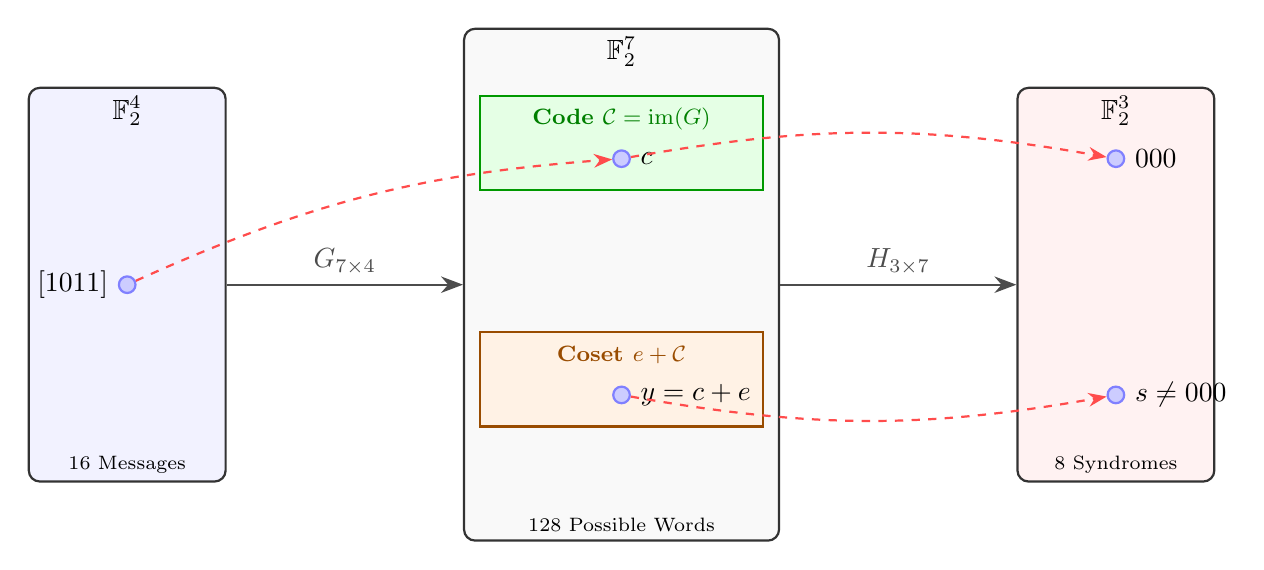
\begin{tikzpicture}[
		font=\sffamily,
		space/.style={draw=black!80, thick, rounded corners, fill=white, inner sep=10pt},
		element/.style={fill=blue!20, draw=blue!50, thick, circle, inner sep=2pt, minimum size=6pt},
		arrow/.style={-{Stealth[scale=1.2]}, thick, black!70},
		mapping/.style={-{Stealth}, dashed, thick, red!70}
		]
		
		% Left: 4-bit Message
		\node[space, minimum width=2.5cm, minimum height=5cm, fill=blue!5] (F4) {};
		\node[anchor=north, font=\bfseries] at (F4.north) {$\mathbb{F}_2^4$};
		\node[anchor=south, font=\scriptsize] at (F4.south) {16 Messages};
		\node[element, label=left:{$[1011]$}] (m) at (F4.center) {};
		
		% Middle: 7-bit Ambient
		\node[space, right=3cm of F4, minimum width=4cm, minimum height=6.5cm, fill=gray!5] (F7) {};
		\node[anchor=north, font=\bfseries] at (F7.north) {$\mathbb{F}_2^7$};
		\node[anchor=south, font=\scriptsize] at (F7.south) {128 Possible Words};
		
		% Valid Code Subspace
		\draw[draw=green!60!black, thick, fill=green!10] 
		($(F7.center) + (-1.8, 1.2)$) rectangle ($(F7.center) + (1.8, 2.4)$);
		\node[font=\footnotesize\bfseries, green!50!black] at ($(F7.center) + (0, 2.1)$) {Code $\mathcal{C} = \mathrm{im}(G)$};
		\node[element, label=right:{$c$}] (c) at ($(F7.center) + (0, 1.6)$) {};
		
		% Error Coset
		\draw[draw=orange!60!black, thick, fill=orange!10] 
		($(F7.center) + (-1.8, -1.8)$) rectangle ($(F7.center) + (1.8, -0.6)$);
		\node[font=\footnotesize\bfseries, orange!60!black] at ($(F7.center) + (0, -0.9)$) {Coset $e + \mathcal{C}$};
		\node[element, label=right:{$y = c+e$}] (y) at ($(F7.center) + (0, -1.4)$) {};
		
		% Right: 3-bit Syndrome
		\node[space, right=3cm of F7, minimum width=2.5cm, minimum height=5cm, fill=red!5] (F3) {};
		\node[anchor=north, font=\bfseries] at (F3.north) {$\mathbb{F}_2^3$};
		\node[anchor=south, font=\scriptsize] at (F3.south) {8 Syndromes};
		
		\node[element, label=right:{$000$}] (s0) at ($(F3.center) + (0, 1.6)$) {};
		\node[element, label=right:{$s \neq 000$}] (synd) at ($(F3.center) + (0, -1.4)$) {};
		
		% Mappings
		\draw[arrow] (F4) -- (F7) node[midway, above] {$G_{7 \times 4}$};
		\draw[arrow] (F7) -- (F3) node[midway, above] {$H_{3 \times 7}$};
		
		\draw[mapping] (m) to[bend left=10] (c);
		\draw[mapping] (c) to[bend left=10] (s0);
		\draw[mapping] (y) to[bend right=10] (synd);
		
	\end{tikzpicture}
\end{document}